% Documentclass options:
%    10pt, 11pt, 12pt  -- set type size
%    draft             -- single space, mark overfull hboxes on paper
%    final             -- double space, don't mark overfull hboxes on paper
%    oneside           -- format for one-sided printing
%    twoside           -- format for two-sided printing
% Defaults are 11pt,final,oneside.  Keep these, please.
\documentclass[11pt]{ucscthesisbs}
\bibliographystyle{apalike2}
\usepackage{natbib}
\usepackage{graphicx,epsf}% Include figure files
\usepackage{pgfplots} %for doing graphics within latex!

% The following declaration is for citations and bibliographies consistent with
% Astrophysical Journal specifications.  It may be left out or replaced with
% another bibliography/citation style.  See also the "\bibliographystyle"
% command later in this file.
%\usepackage{apj}

\usepackage{xcolor}
\usepackage{pagecolor}
\usepackage{lipsum}  

\pagecolor{darkgray}
\color{white}

% \pagecolor{white}
% \color{black}


\begin{document}

% Declarations for Front Matter

\title{Condensation-inhibited convection in the atmosphere of uranus and its impact on thermal evolution}
\author{Robert Schroder}
\degreeyear{2020}
\degreemonth{27 November}
\degree{BACHELOR OF SCIENCE}
\field{ASTROPHYSICS}%
% Declare up to five committee members.  The text will be reproduced directly
% on the signature page.  Though the chair is a committee member, leave
% him/her out of the \committeemember declarations.  Make sure \numberofmembers
% agrees with the number of committee members declared INCLUDING the chair.
% If it is wrong, you will get extra or missing lines on the signature page.
%
\chair{Professor Bruce Schumm}
\technicaladvisor{Christopher Mankovich}


\campus{Santa Cruz}

\maketitle
\copyrightpage

\begin{frontmatter}

\begin{abstract}
This will be the last section written, once we have finished our analysis.
\end{abstract}

\tableofcontents
%
% The most recent (10/95) guidelines make absolutely no mention of the list
% of figures and list of tables.  Are they necessary?  If not, comment the
% next two lines out.
%
\listoffigures
\listoftables

\begin{dedication}
\null\vfil
{\large
\begin{center}
To my wife,\\\vspace{12pt}
Stinkers
\end{center}}
\vfil\null
\end{dedication}

\begin{acknowledgements}

\end{acknowledgements}


\end{frontmatter}

%\part{First Part}

\chapter{Introduction}
As planets coalesce from their protoplanetary disk, they heat from the release of gravitational potential energy. Eventually, they stop collapsing when they reach hydrostatic equilibrium, and then the process of cooling begins as they release this latent heat of formation through the tops of their atmosphere. There are deviations from this trend, as when terrestrial planets undergo a greenhouse effect, or warm due to the formation of a secondary atmosphere caused by outgassing of cooling molten material. Planets, both terrestrial and giant, may migrate closer to their parent star, increasing the amount of stellar radiation absorbed by the planet's atmosphere. In our solar system, the giant planets are far from the Sun, quite old, and primarily of solar composition. As such, we are not concerned with those warming scenarios here. In this paper, we examine the thermal evolution of the planet Uranus. Uranus is closer to the Sun than its neighbor Neptune, with which it shares similarities in mass and chemical composition. Oddly, it is cooler than its more distant counterpart. Much work has been done with model Uranus atmospheres. These models assume a thoroughly convective atmosphere and have been consistently at odds with observation and do not predict the under-luminous Uranus that we now observe. In this paper, we examine the impact of condensation-inhibited convection on the planet's thermal evolution to see if it offers a possible explanation for current observations. In section 1.1, we review prior work done on model atmospheres of solar system giant planets. In section 1.2, we review prior work done on the formation of water condensation zones in these hydrogen rich atmospheres. In chapter 2, we describe our model and discuss the ramifications for the thermal evolution of Uranus.



\section{Model Atmospheres}

Will review current understanding of solar system giant planet thermal evolution here, referencing work done by Fortney, et al., and others. Not sure how far back I want to go here, but will probably mention when, and by who, thermal evolution modeling began, and then quickly get into the thermal evolution background from fortney papers.


\section{Condensation-inhibited Convection}\label{subsection_example}

% When you cite a reference as the source for a piece of information,
% you generally place it just after you give the information, using the "citep"
% command \citep{awwzml06}.  However, sometimes you want to refer directly to 
% the authors, as \citet{agcs89} did several times, in which case you use "citet".
% We are using the American Psychological Association conventions for citations
% (what appears in the text) and references (what appears in the bibiography in
% the end).  Of course every citation must correspond to a reference and vice versa.

This section will contain theory surrounding condensation in hydrogen rich atmospheres, citing LeConte, Friedson, others.

\begin{figure}[t!]
 \centerline{
  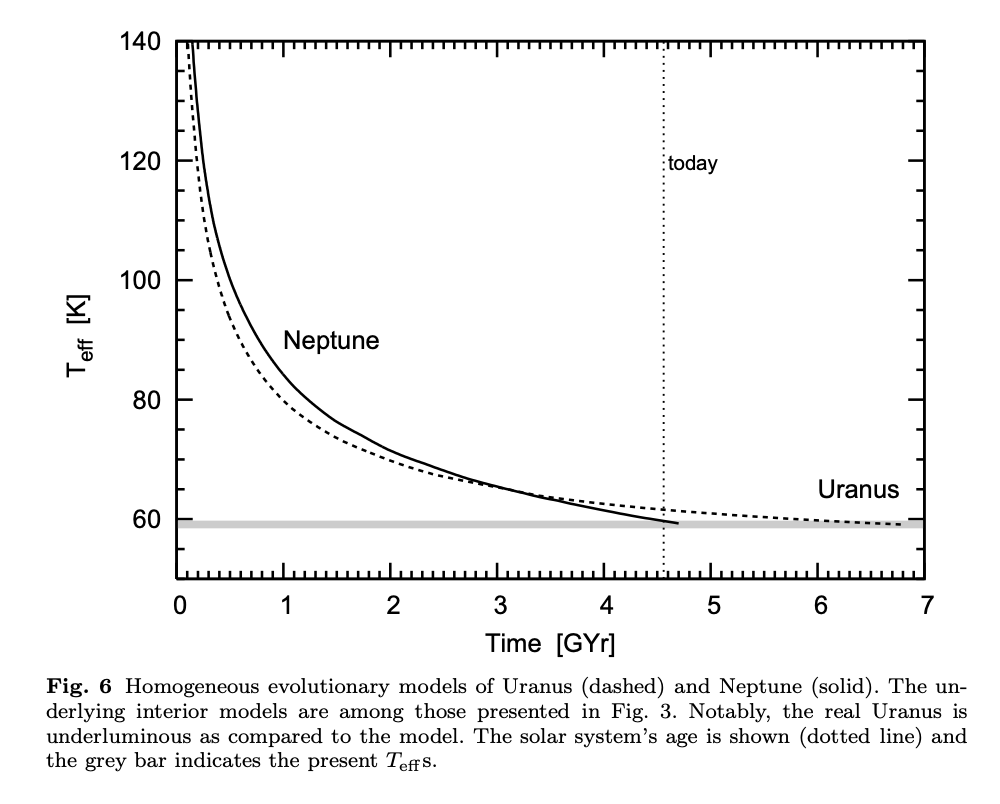
\includegraphics[width=4.0in]{fortney_nettelmann2010_UN_curves.png}
 }
\caption[Transverse Scans at difference Temperatures at $H=11$~T]
{bobloblaw 
}
\label{fig:discretescan}
\end{figure}

\section{Open Questions}\label{open_questions}
Describe where the current models fail (ex: uranus, neptune, saturn)



\subsection{A subsection on tables}\label{tables}

Not only do I give two examples on tables here, I show you how to force tables (or other "floating" environments like figures) to appear close to where you want them.

When I first compiled this, the tables meant for this section appeared during the following one.  LaTeX is just trying to arrange things well and avoid blank space, but if you want to prioritize having something appear about where you put it in the LaTeX code, put the notation 
"{\tt [!htb]}" as shown at the start of the tables here.  The "h" stands for "put it here,"  The "h" stands for "here," the "t" for "top," the "b" for "bottom," and the "!" for something like, "really, darnit, override some rules if you have to.  You can use "b" or "t" alone or with the "!" if you like to see all your figures at the top of a page (common) or at the bottom (rare).  

Note that if your placement choices end up generating a lot of whitespace, that whitespace will not count toward the minimum page count of your thesis.

\begin{table}[!htb]
\centerline{
\begin{tabular}{|l|r|}
  \hline 
Title & Author \\
\hline
War And Peace & Leo Tolstoy \\
The Great Gatsby & F. Scott Fitzgerald \\ \hline
\end{tabular}
}
\caption{A normalsize table.  This would be the normal size that you would make a table, so that it is most readable, unless it's hard to fit everything in.  Some journals (like Physical Review) use captions at the bottom of tables that can be as wordy as the caption to a figure, like this one.  If your thesis is in physics or applied physics, rather than astrophysics, you should use this convention.}
\end{table}

\begin{table}[!htb]
\caption{A small table.$^a$}
\centerline{
\begin{scriptsizetabular}{|l|r|}
  \hline 
Title & Author \\
\hline
War And Peace & Leo Tolstoy \\
The Great Gatsby$^b$ & F. Scott Fitzgerald \\ \hline
\end{scriptsizetabular}
}

\begin{quote}  %I'm using the quote environment to get single spacing.
$^a$In astrophysics, the table title is usually short and always at the top, and other information is put into table footnotes like this.

$^b$ A much shorter read than War and Peace.
\end{quote}

\end{table}

\subsection{Graphics with pgfplots}

\pgfmathdeclarefunction{gauss}{2}{%
  \pgfmathparse{1/(#2*sqrt(2*pi))*exp(-((x-#1)^2)/(2*#2^2))}%
}

\begin{figure}\label{agraphic}
\centering
\begin{tikzpicture}
\begin{axis}[
  no markers, domain=0:10, samples=100,
  axis lines*=left, xlabel=$x$, ylabel=$y$,
  every axis y label/.style={at=(current axis.above origin),anchor=south},
  every axis x label/.style={at=(current axis.right of origin),anchor=west},
  height=5cm, width=12cm,
  xtick={4,6.5}, ytick=\empty,
  enlargelimits=false, clip=false, axis on top,
  grid = major
  ]
  \addplot [fill=cyan!20, draw=none, domain=0:5.96] {gauss(6.5,1)} \closedcycle;
  \addplot [very thick,cyan!50!black] {gauss(4,1)};
  \addplot [very thick,cyan!50!black] {gauss(6.5,1)};
\draw [yshift=-0.6cm, latex-latex](axis cs:4,0) -- node [fill=white] {$1.96\sigma$} (axis cs:5.96,0);
\end{axis}
\end{tikzpicture}
\caption{This graphic was generated using the pdfplots package, which is a wrapper for a more fundamental LaTeX package called "tikz".  }
\end{figure}

In this subsection I show an example of how to create plots {\it within} LaTeX, using a package called "pgfplots".  I have verified that it works in Overleaf.  If you are compiling elsewhere and get an error that the package is unknown, you can either get it at 
\begin{center}
{\tt http://pgfplots.sourceforge.net/}
\end{center}
or else remove the reference to the package from the preamble of this document and remove the {\tt tikzpicture} block from this subsection.



\chapter{Previous Work}

This section contains another figure, this one a .jpg file; it is Figure~\ref{fig:jpgfile}.

Some other research was once performed.
Some other research was once performed.
Some other research was once performed.
Some other research was once performed.
Some other research was once performed.
Some other research was once performed.
Some other research was once performed.
Some other research was once performed.
Some other research was once performed.
Some other research was once performed.
Some other research was once performed.

Some other research was once performed.
Some other research was once performed.
Some other research was once performed.
Some other research was once performed.
Some other research was once performed.
Some other research was once performed.
Some other research was once performed.
Some other research was once performed.

\begin{figure}[t!]
 \centerline{
  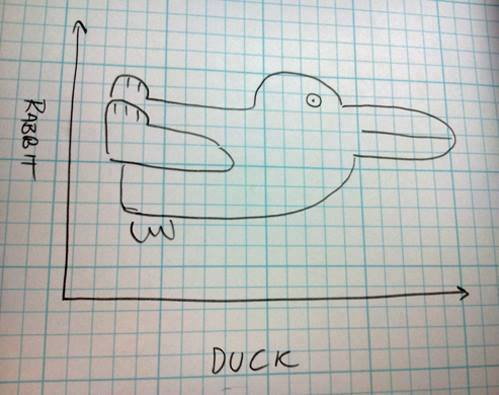
\includegraphics[width=4.0in]{rabbit-or-duck.jpg}
 }
\caption[Rabbit or duck?]
{An image that looks like a rabbit one way, and a duck another.  Your caption should describe everything that the reader sees looking at the figure, but {\it interpretation and significance} should be left for the main text.
}
\label{fig:jpgfile}
\end{figure}

\chapter{Conclusion}

I actually don't like to use "conclusion" for the final section, as it's not clear on the purpose.  I think it's better to have a "discussion" and a "summary".  In the discussion, you bring up new information by {\it interpreting} your result in the context of theory and other peoples' work; this can include new ideas and new citations.  In the summary, which will be very much like the abstract, you simply sum up your main conclusions (although the abstract, unlike the summary, has to briefly define the problem and methods).

This is where a conclusion would go.
This is where a conclusion would go.
This is where a conclusion would go.
This is where a conclusion would go.
This is where a conclusion would go.
This is where a conclusion would go.
This is where a conclusion would go.
This is where a conclusion would go.
This is where a conclusion would go.
This is where a conclusion would go.
This is where a conclusion would go.

This is where a conclusion would go.
This is where a conclusion would go.
This is where a conclusion would go.
This is where a conclusion would go.
This is where a conclusion would go.
This is where a conclusion would go.
This is where a conclusion would go.
This is where a conclusion would go.

This is where a conclusion would go.
This is where a conclusion would go.
This is where a conclusion would go.
This is where a conclusion would go.
This is where a conclusion would go.
This is where a conclusion would go.
This is where a conclusion would go.
This is where a conclusion would go.

\appendix
\chapter{Some Ancillary Stuff}

Ancillary material should be put in appendices.  The guidelines are not
clear whether bibliography comes before or after the appendices, but they
\emph{suggest} appendices come first.
Ancillary material should be put in appendices.  The guidelines are not
clear whether bibliography comes before or after the appendices, but they
\emph{suggest} appendices come first.
Ancillary material should be put in appendices.  The guidelines are not
clear whether bibliography comes before or after the appendices, but they
\emph{suggest} appendices come first.
Ancillary material should be put in appendices.  The guidelines are not
clear whether bibliography comes before or after the appendices, but they
\emph{suggest} appendices come first.

%\nocite{*}

\bibliography{magnetism}

%\begin{thebibliography}{999}
%\bibitem{spa02}E. T. Sepp\"{al}\"{a}, A. M. Pulkkinen, and M. J. Alava,
%Phys.\ Rev.\ B {\bf 66}, 144403 (2002).
%\end{thebibliography}

\end{document}
